\section{Revisão Bibliográfica}

Redes Neurais Artificiais são técnicas computacionais que apresentam um modelo matemático inspirado na estrutura neural de organismos inteligentes e que adquirem conhecimento através da experiência. A arquitetura base de rede neural estudada neste artigo é a Perceptron de Múltiplas Camadas (do inglês, Multilayer Perceptron, ou apenas MLP).

\subsection{Perceptrom de Multiplas Camadas}

Uma rede MLP consiste em pelo menos três camadas: uma camada de entrada, uma camada oculta e uma camada de saída. O MLP utiliza uma técnica de aprendizado supervisionada chamada \textit{backpropagation} para treinamento.


\begin{figure}[h!]

\centering % para centralizarmos a figura
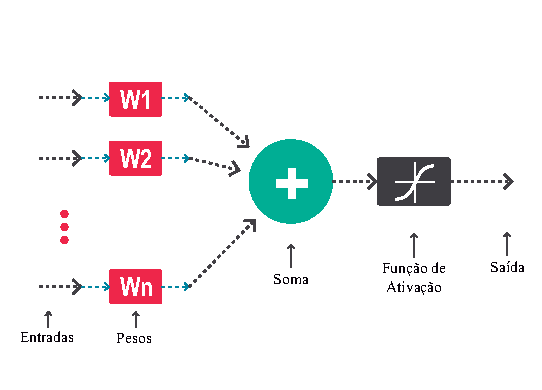
\includegraphics{04-Figuras/Arquitetura}

\caption{Arquitetura de uma rede MLP}

\label{figura:arquitetura}

\end{figure}

A fig.{label:arquitetura} mostra

In convallis. Fusce suscipit libero eget elit. Praesent vitae arcu tempor neque lacinia pretium. Morbi imperdiet, mauris ac auctor dictum, nisl ligula egestas nulla, et sollicitudin sem purus in lacus.



Morbi a metus. Phasellus enim erat, vestibulum vel, aliquam a, posuere eu, velit. Nullam sapien sem, ornare ac, nonummy non, lobortis a, enim. Nunc tincidunt ante vitae massa. Duis ante orci, molestie vitae, vehicula venenatis, tincidunt ac, pede. Nulla accumsan, elit sit amet varius semper, nulla mauris mollis quam, tempor suscipit diam nulla vel leo. Etiam commodo dui eget wisi. Donec iaculis gravida nulla. Donec quis nibh at felis congue commodo. Etiam bibendum elit eget erat.

\subsection{Algoritmo Backpropagation}

Nam quis nulla. Integer malesuada. In in enim a arcu imperdiet malesuada. Sed vel lectus. Donec odio urna, tempus molestie, porttitor ut, iaculis quis, sem. Phasellus rhoncus. Aenean id metus id velit ullamcorper pulvinar. Vestibulum fermentum tortor id mi. Pellentesque ipsum. Nulla non arcu lacinia neque faucibus fringilla. Nulla non lectus sed nisl molestie malesuada. Proin in tellus sit amet nibh dignissim sagittis. Vivamus luctus egestas leo. Maecenas sollicitudin. Nullam rhoncus aliquam metus. Etiam egestas wisi a erat.

Maecenas ipsum velit, consectetuer eu, lobortis ut, dictum at, dui. In rutrum. Sed ac dolor sit amet purus malesuada congue. In laoreet, magna id viverra tincidunt, sem odio bibendum justo, vel imperdiet sapien wisi sed libero. Suspendisse sagittis ultrices augue. Mauris metus. Nunc dapibus tortor vel mi dapibus sollicitudin. Etiam posuere lacus quis dolor. Praesent id justo in neque elementum ultrices. Class aptent taciti sociosqu ad litora torquent per conubia nostra, per inceptos hymenaeos. In convallis. Fusce suscipit libero eget elit. Praesent vitae arcu tempor neque lacinia pretium. Morbi imperdiet, mauris ac auctor dictum, nisl ligula egestas nulla, et sollicitudin sem purus in lacus.

Aenean placerat. In vulputate urna eu arcu. Aliquam erat volutpat. Suspendisse potenti. Morbi mattis felis at nunc. Duis viverra diam non justo. In nisl. Nullam sit amet magna in magna gravida vehicula. Mauris tincidunt sem sed arcu. Nunc posuere. Nullam lectus justo, vulputate eget, mollis sed, tempor sed, magna. Cum sociis natoque penatibus et magnis dis parturient montes, nascetur ridiculus mus. Etiam neque. Curabitur ligula sapien, pulvinar a, vestibulum quis, facilisis vel, sapien. Nullam eget nisl. Donec vitae arcu.

\subsection{Estrutura Competitiva Auto Associativa}

Maecenas ipsum velit, consectetuer eu, lobortis ut, dictum at, dui. In rutrum. Sed ac dolor sit amet purus malesuada congue. In laoreet, magna id viverra tincidunt, sem odio bibendum justo, vel imperdiet sapien wisi sed libero. Suspendisse sagittis ultrices augue. Mauris metus. Nunc dapibus tortor vel mi dapibus sollicitudin. Etiam posuere lacus quis dolor. Praesent id justo in neque elementum ultrices. Class aptent taciti sociosqu ad litora torquent per conubia nostra, per inceptos hymenaeos. In convallis. Fusce suscipit libero eget elit. Praesent vitae arcu tempor neque lacinia pretium. Morbi imperdiet, mauris ac auctor dictum, nisl ligula egestas nulla, et sollicitudin sem purus in lacus.



Aenean placerat. In vulputate urna eu arcu. Aliquam erat volutpat. Suspendisse potenti. Morbi mattis felis at nunc. Duis viverra diam non justo. In nisl. Nullam sit amet magna in magna gravida vehicula. Mauris tincidunt sem sed arcu. Nunc posuere. Nullam lectus justo, vulputate eget, mollis sed, tempor sed, magna. Cum sociis natoque penatibus et magnis dis parturient montes, nascetur ridiculus mus. Etiam neque. Curabitur ligula sapien, pulvinar a, vestibulum quis, facilisis vel, sapien. Nullam eget nisl. Donec vitae arcu.

Morbi a metus. Phasellus enim erat, vestibulum vel, aliquam a, posuere eu, velit. Nullam sapien sem, ornare ac, nonummy non, lobortis a, enim. Nunc tincidunt ante vitae massa. Duis ante orci, molestie vitae, vehicula venenatis, tincidunt ac, pede. Nulla accumsan, elit sit amet varius semper, nulla mauris mollis quam, tempor suscipit diam nulla vel leo. Etiam commodo dui eget wisi. Donec iaculis gravida nulla. Donec quis nibh at felis congue commodo. Etiam bibendum elit eget erat.

Nam quis nulla. Integer malesuada. In in enim a arcu imperdiet malesuada. Sed vel lectus. Donec odio urna, tempus molestie, porttitor ut, iaculis quis, sem. Phasellus rhoncus. Aenean id metus id velit ullamcorper pulvinar. Vestibulum fermentum tortor id mi. Pellentesque ipsum. Nulla non arcu lacinia neque faucibus fringilla. Nulla non lectus sed nisl molestie malesuada. Proin in tellus sit amet nibh dignissim sagittis. Vivamus luctus egestas leo. Maecenas sollicitudin. Nullam rhoncus aliquam metus. Etiam egestas wisi a erat.

%=================================================================================================
%=================================================================================================

\section{Desenvolvimento da Rede MPL}

Maecenas ipsum velit, consectetuer eu, lobortis ut, dictum at, dui. In rutrum. Sed ac dolor sit amet purus malesuada congue. In laoreet, magna id viverra tincidunt, sem odio bibendum justo, vel imperdiet sapien wisi sed libero. Suspendisse sagittis ultrices augue. Mauris metus. Nunc dapibus tortor vel mi dapibus sollicitudin. Etiam posuere lacus quis dolor. Praesent id justo in neque elementum ultrices. Class aptent taciti sociosqu ad litora torquent per conubia nostra, per inceptos hymenaeos. In convallis. Fusce suscipit libero eget elit. Praesent vitae arcu tempor neque lacinia pretium. Morbi imperdiet, mauris ac auctor dictum, nisl ligula egestas nulla, et sollicitudin sem purus in lacus.

\begin{figure}[h!]

\centering % para centralizarmos a figura
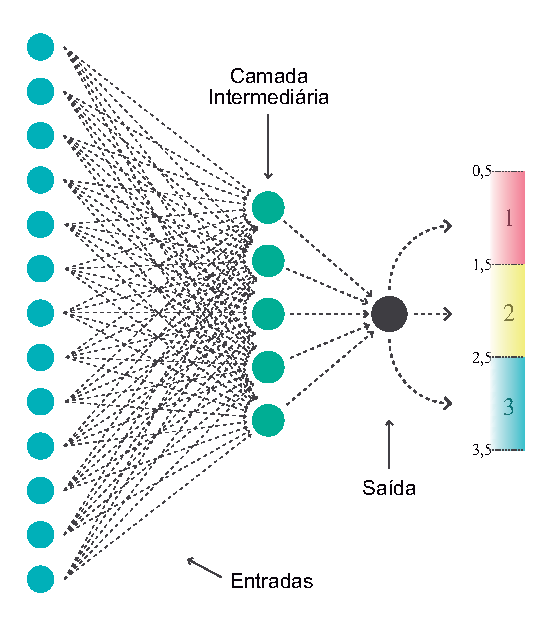
\includegraphics{04-Figuras/Arquitetura-MPL}

\caption{Arquitetura da rede MPL}

\label{figura:arquiteturaMPL}

\end{figure}


\subsection{Ambiente da Aplicação}

Aenean placerat. In vulputate urna eu arcu. Aliquam erat volutpat. Suspendisse potenti. Morbi mattis felis at nunc. Duis viverra diam non justo. In nisl. Nullam sit amet magna in magna gravida vehicula. Mauris tincidunt sem sed arcu. Nunc posuere. Nullam lectus justo, vulputate eget, mollis sed, tempor sed, magna. Cum sociis natoque penatibus et magnis dis parturient montes, nascetur ridiculus mus. Etiam neque. Curabitur ligula sapien, pulvinar a, vestibulum quis, facilisis vel, sapien. Nullam eget nisl. Donec vitae arcu.


\subsection{Base de Dados}

Nam quis nulla. Integer malesuada. In in enim a arcu imperdiet malesuada. Sed vel lectus. Donec odio urna, tempus molestie, porttitor ut, iaculis quis, sem. Phasellus rhoncus. Aenean id metus id velit ullamcorper pulvinar. Vestibulum fermentum tortor id mi. Pellentesque ipsum. Nulla non arcu lacinia neque faucibus fringilla. Nulla non lectus sed nisl molestie malesuada. Proin in tellus sit amet nibh dignissim sagittis. Vivamus luctus egestas leo. Maecenas sollicitudin. Nullam rhoncus aliquam metus. Etiam egestas wisi a erat.


\subsection{Parâmetros de Classificação}

Aenean placerat. In vulputate urna eu arcu. Aliquam erat volutpat. Suspendisse potenti. Morbi mattis felis at nunc. Duis viverra diam non justo. In nisl. Nullam sit amet magna in magna gravida vehicula. Mauris tincidunt sem sed arcu. Nunc posuere. Nullam lectus justo, vulputate eget, mollis sed, tempor sed, magna. Cum sociis natoque penatibus et magnis dis parturient montes, nascetur ridiculus mus. Etiam neque. Curabitur ligula sapien, pulvinar a, vestibulum quis, facilisis vel, sapien. Nullam eget nisl. Donec vitae arcu.

%=================================================================================================
%=================================================================================================

\section{Desenvolvimento da Rede Competitiva Auto Associativa}

Nam quis nulla. Integer malesuada. In in enim a arcu imperdiet malesuada. Sed vel lectus. Donec odio urna, tempus molestie, porttitor ut, iaculis quis, sem. Phasellus rhoncus. Aenean id metus id velit ullamcorper pulvinar. Vestibulum fermentum tortor id mi. Pellentesque ipsum. Nulla non arcu lacinia neque faucibus fringilla. Nulla non lectus sed nisl molestie malesuada. Proin in tellus sit amet nibh dignissim sagittis. Vivamus luctus egestas leo. Maecenas sollicitudin. Nullam rhoncus aliquam metus. Etiam egestas wisi a erat.

\subsection{Arquitetura}

Aenean placerat. In vulputate urna eu arcu. Aliquam erat volutpat. Suspendisse potenti. Morbi mattis felis at nunc. Duis viverra diam non justo. In nisl. Nullam sit amet magna in magna gravida vehicula. Mauris tincidunt sem sed arcu. Nunc posuere. Nullam lectus justo, vulputate eget, mollis sed, tempor sed, magna. Cum sociis natoque penatibus et magnis dis parturient montes, nascetur ridiculus mus. Etiam neque. Curabitur ligula sapien, pulvinar a, vestibulum quis, facilisis vel, sapien. Nullam eget nisl. Donec vitae arcu.

\begin{figure}[h!]

\centering % para centralizarmos a figura
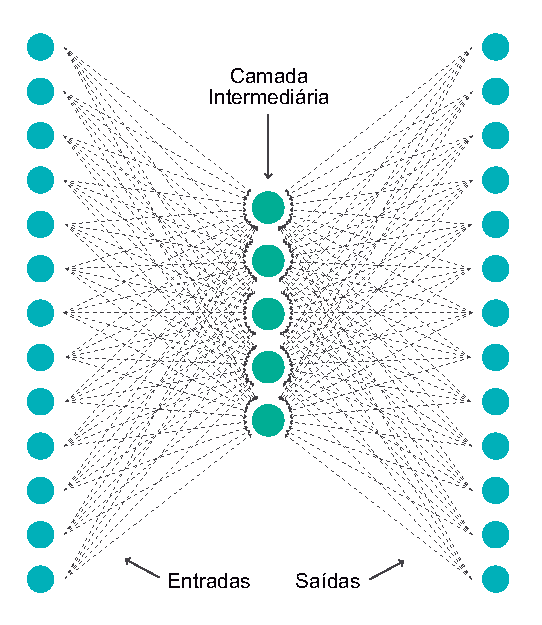
\includegraphics{04-Figuras/Arquitetura-AutoAssociativa}

\caption{Arquitetura da rede Competitiva Auto Associativa}

\label{figura:arquiteturaAuto}

\end{figure}